
\section{Flow区域处理}

Flow区域典型特征就是包含多种方向纹理低灰度条纹, 这使得直接通过门限值过滤方法并不现实. 我们注意到, 在数据中要保留的流场区域的纹理几乎不存在垂直方向, 单背景区域则有大量纵向纹理条纹, 所以我们提出通过纵向纹理抑制,非纵向条纹加深和灰度门限值方法对$V_b$像素进行判别.

具体来说,我们可以通过左右方向的锐化使得非纵向条纹灰度值降低(变黑),纵向条纹灰度模糊(变高),这可通过原图和方向锐化卷积核的卷积实现. 操作后纵向与非纵向条纹的灰度值拉开范围, 这时就可通过灰度值门限的方法较为准确的提取到非纵向纹理的位置, 即可得到$M_f(p)$, 具体公式如下:


\begin{eqnarray}
\nonumber
\quad&I_1(p) = I \ast N&\\
\nonumber
\quad&I_2(p) = I \ast S&\\
\nonumber
\quad&M_f(p) = [I_1(p) \le \delta_1] \oplus [I_2(p) \le \delta_2]&
\end{eqnarray}

其中, $\ast$为图像卷积操作, $[\cdot]$为 Iverson 算符\footnote{[1+1=3]=0;
[1+1=2]=1}, $\oplus$ 为二元或运算, N和S为方向卷积核, 值分别为:

\begin{eqnarray}
	\nonumber
	N = \left(                
		\begin{array}{ccc} 
		  1 & 2 & 1\\  
		  0 & 1 & 0\\  
		  -1&-2&-1\\
		\end{array}
	  \right) \\
	  \nonumber
	  S = \left(                
		  \begin{array}{ccc} 
			-1 & -2 & -1\\  
			0 & 1 & 0\\  
			1&2&1\\
		  \end{array}
		\right) 
\end{eqnarray}
 通过上述操作, 可得到图.\ref{fig:Mf}.
\begin{figure}[t]
	\begin{center}
		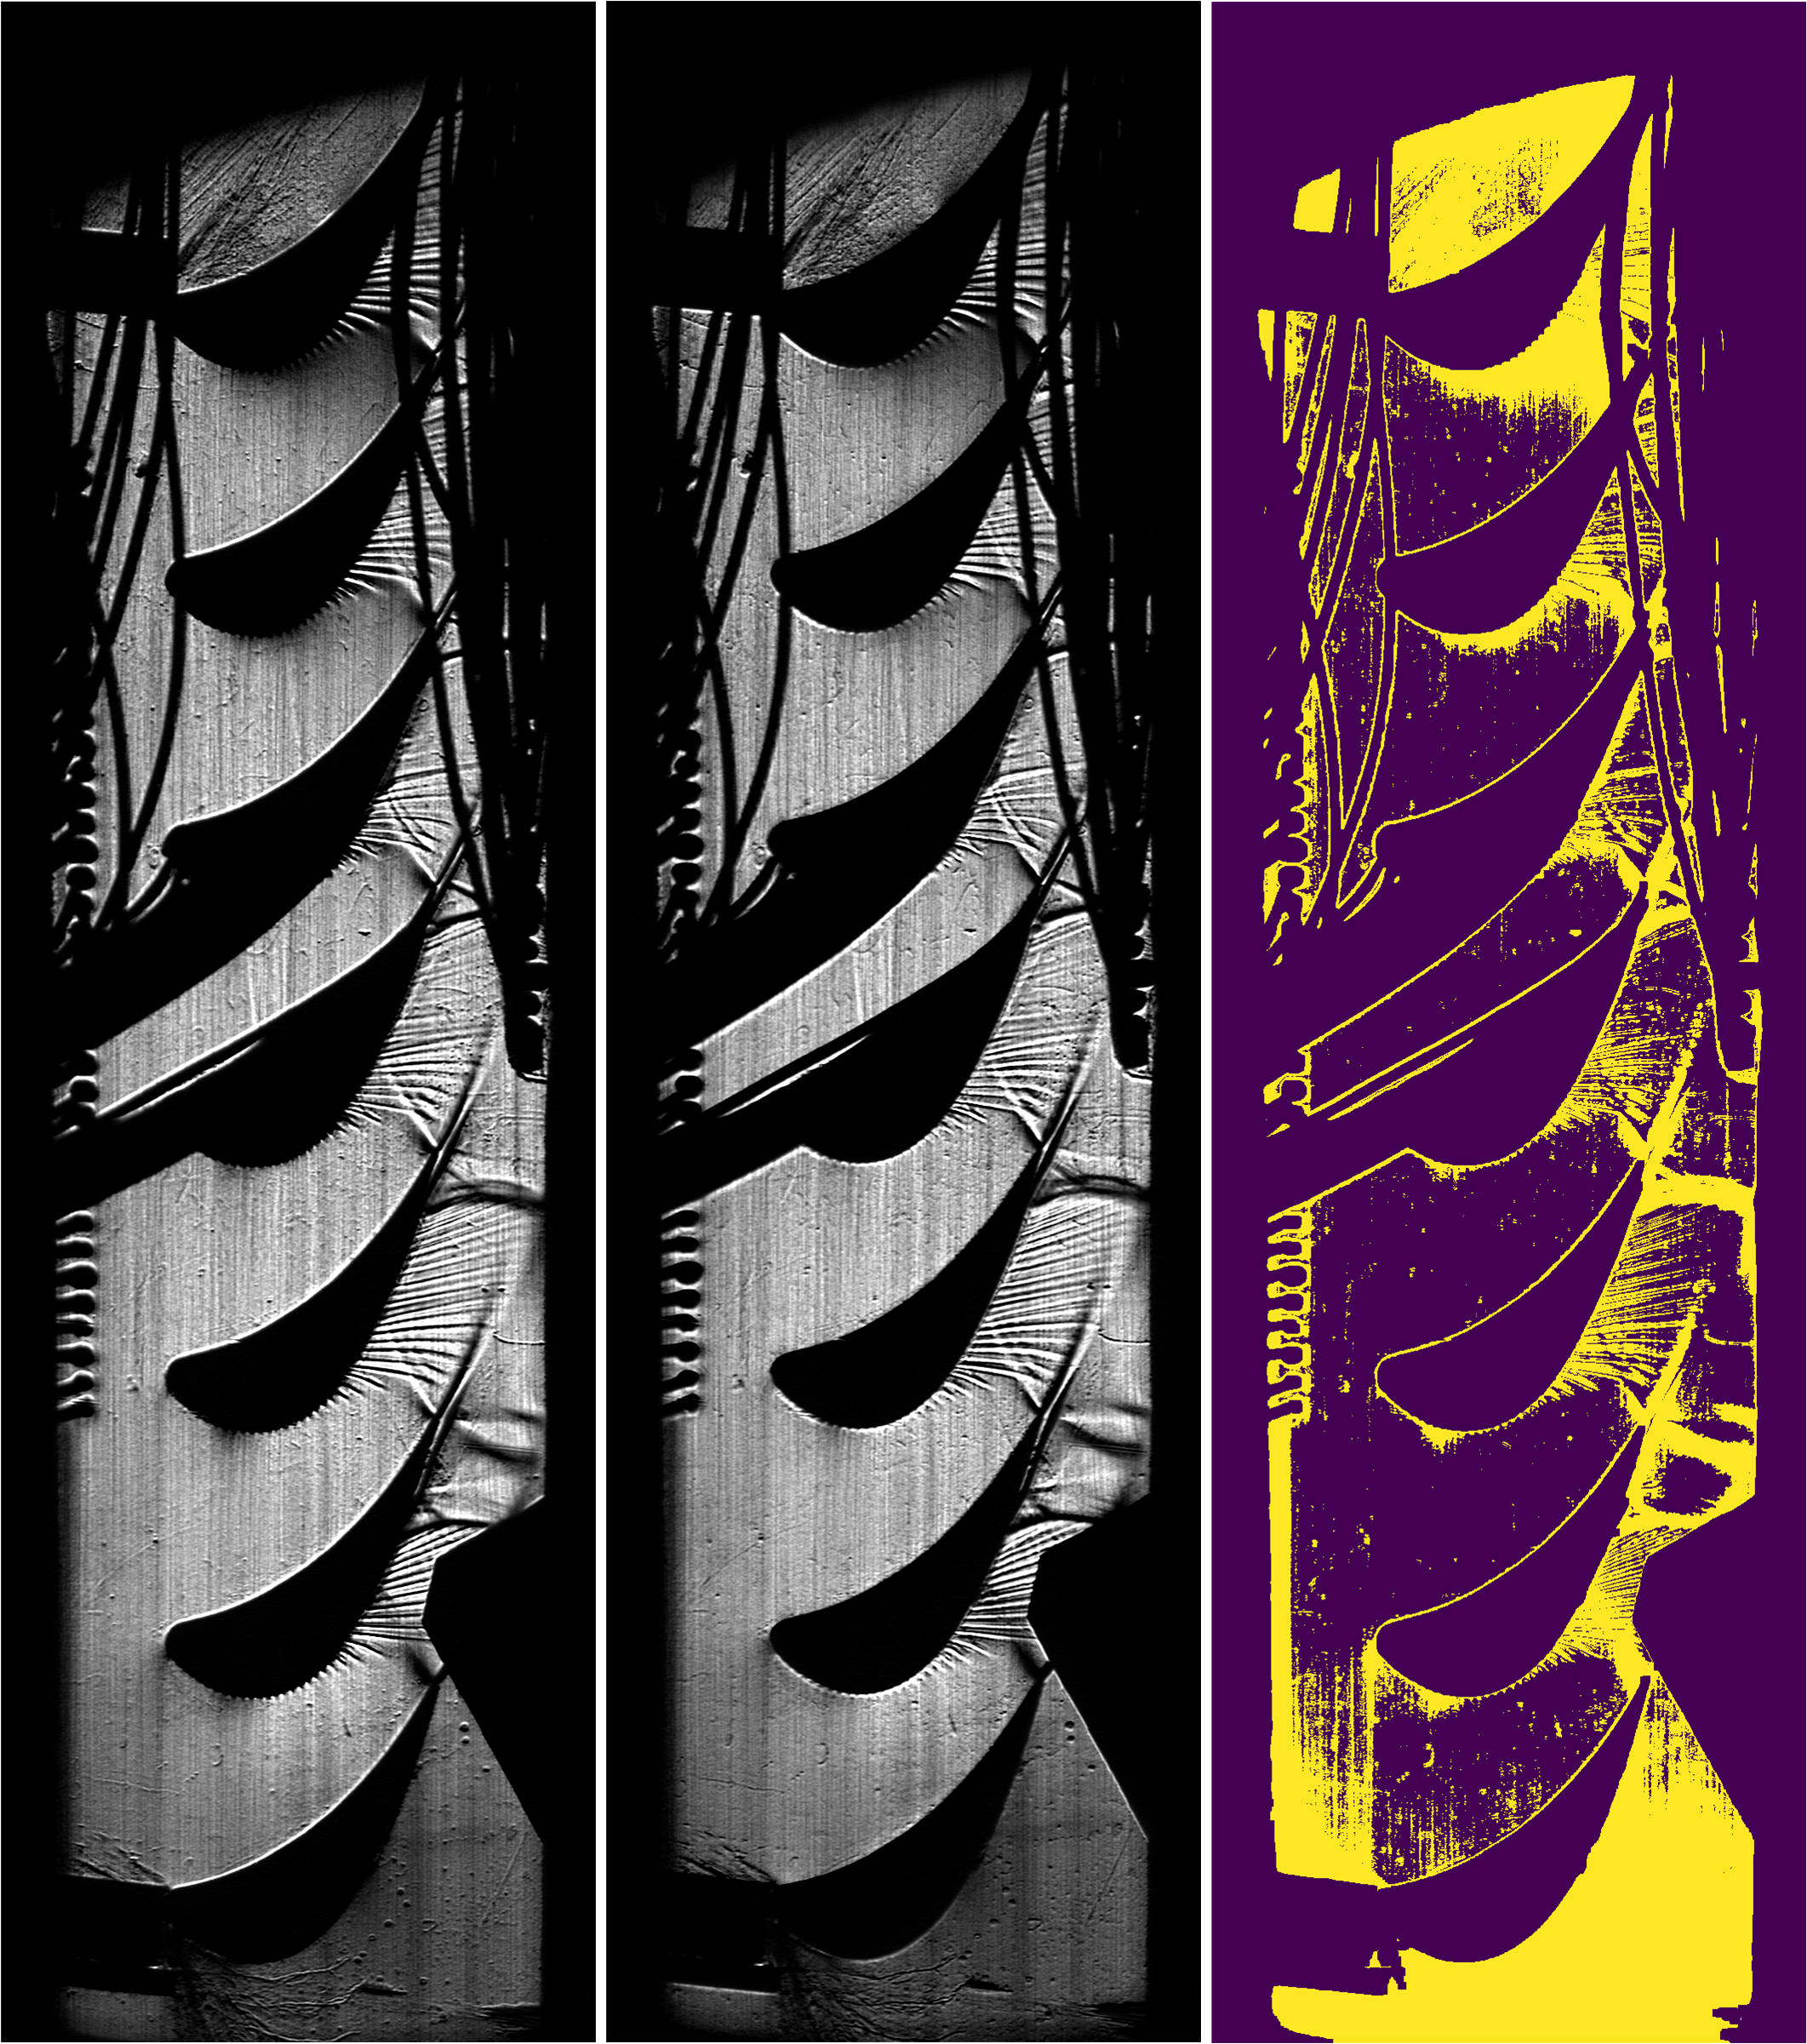
\includegraphics[width=0.75\linewidth]{src/Mf}
	\end{center}
	\caption{ 从左到右依次分别是$I_n$, $I_s$,$M_f$.}
	\label{fig:Mf}	
\end{figure}



